\section{Área de Estudio}

\subsection{Ubicación Geográfica}

% Descripción precisa con coordenadas
Este proyecto se realizara sobre un sector del pais de Chile conocido como "Región Metropolitana de Santiago", la cual es una de las 16 divisiones territoriales de alto nivel denominadas regiones; Se encuentra ubicada en la zona central de Chile, entre los 32°55' y 34°19' de latitud sur, y entre los 69°46' y 71°43' de longitud oeste.\\
Con una superficie de 15,403.2 km² es la única región chilena que no tiene litoral (costas) y se encuentra rodeada por otras regiones y países: al norte y oeste limita con la Región de Valparaíso, al sur con la Región del Libertador General Bernardo O'Higgins, y al este con la República Argentina.\\
Su capital es Santiago de Chile, que también es la capital nacional. Geográficamente, la región se caracteriza por una depresión intermedia, conocida como el Valle de Santiago, que está rodeada por la Cordillera de los Andes al este y la Cordillera de la Costa al oeste.

\begin{figure}[H]
    \centering
    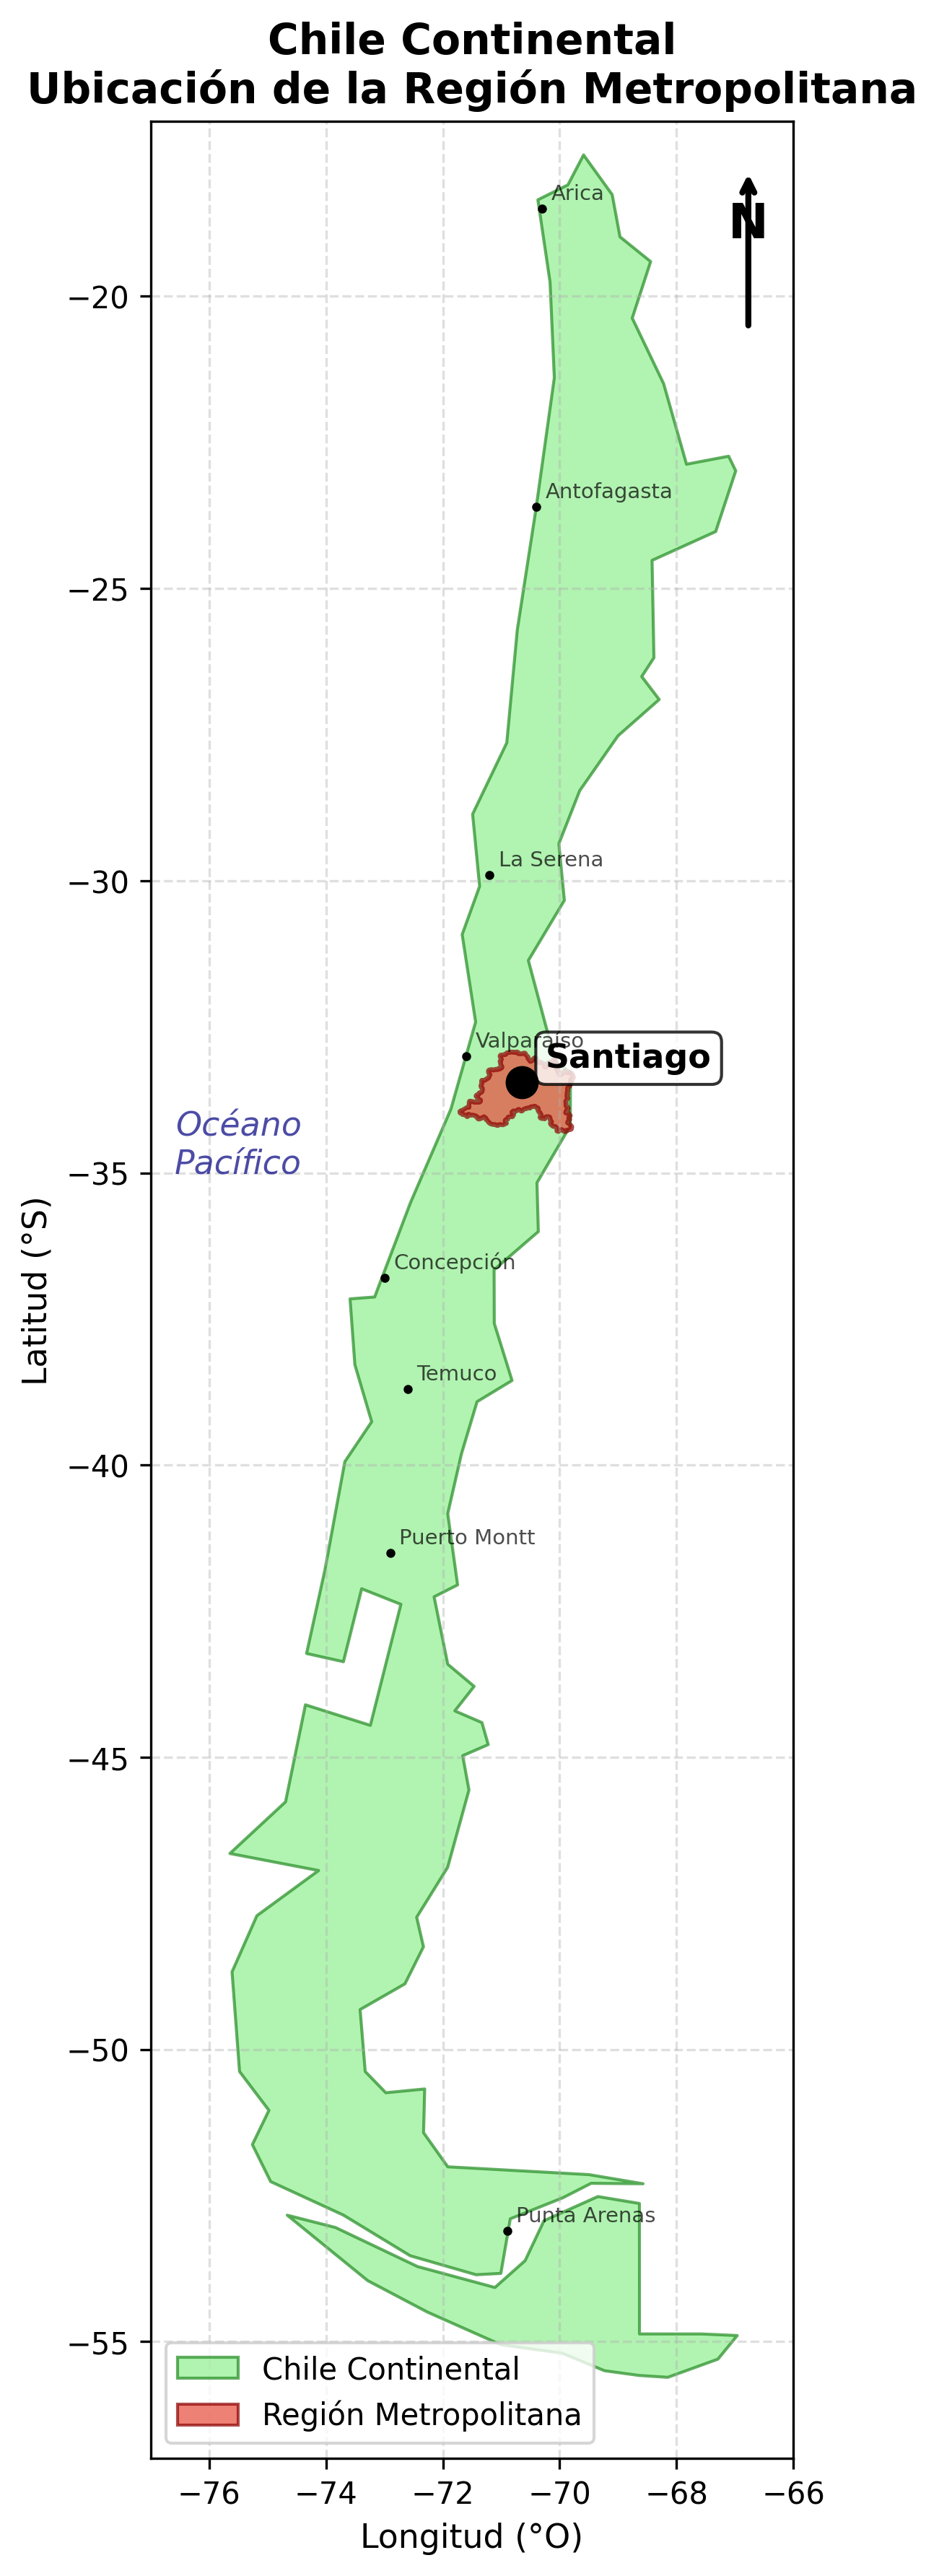
\includegraphics[width=0.2\textwidth]{figuras/figura1_chile_rm.png}
    \caption{Mapa ubicación Región Metropolitana de Santiago}
    \label{fig:ubicacion}
\end{figure}

Debido al alcance reducido del proyecto solo se consideraran las siguientes cuatro comunas dentro la Región Metropolitana de Santiago como parte del área de estudio.

\begin{table}[H]
\centering
\caption{Comunas alcance área de estudio}
\label{tab:comunas}
\begin{tabular}{@{}llll@{}}
\toprule
\textbf{Nombre Comuna} & \textbf{Coordenadas} & \textbf{Superficie total (km²)} & \textbf{Altura promedio (m)}\\
\midrule 
Estación Central & $33^\circ 27' 07''\mathrm{S} \quad 70^\circ 40' 44''\mathrm{O}$ & 14.1 & 512\\
La Reina &  $33^\circ 27' 00''\mathrm{S} \quad 70^\circ 33' 00''\mathrm{O}$ & 23.4 & 680\\
Ñuñoa &  $33^\circ 28' 00''\mathrm{S} \quad 70^\circ 36' 00''\mathrm{O}$ & 16.9 & 560\\
Santiago Centro &  $33^\circ 27' 00''\mathrm{S} \quad 70^\circ 40' 00''\mathrm{O}$ & 22.4 & 520\\
\bottomrule
\end{tabular}
\end{table}
    
\begin{figure}[H]
    \centering
    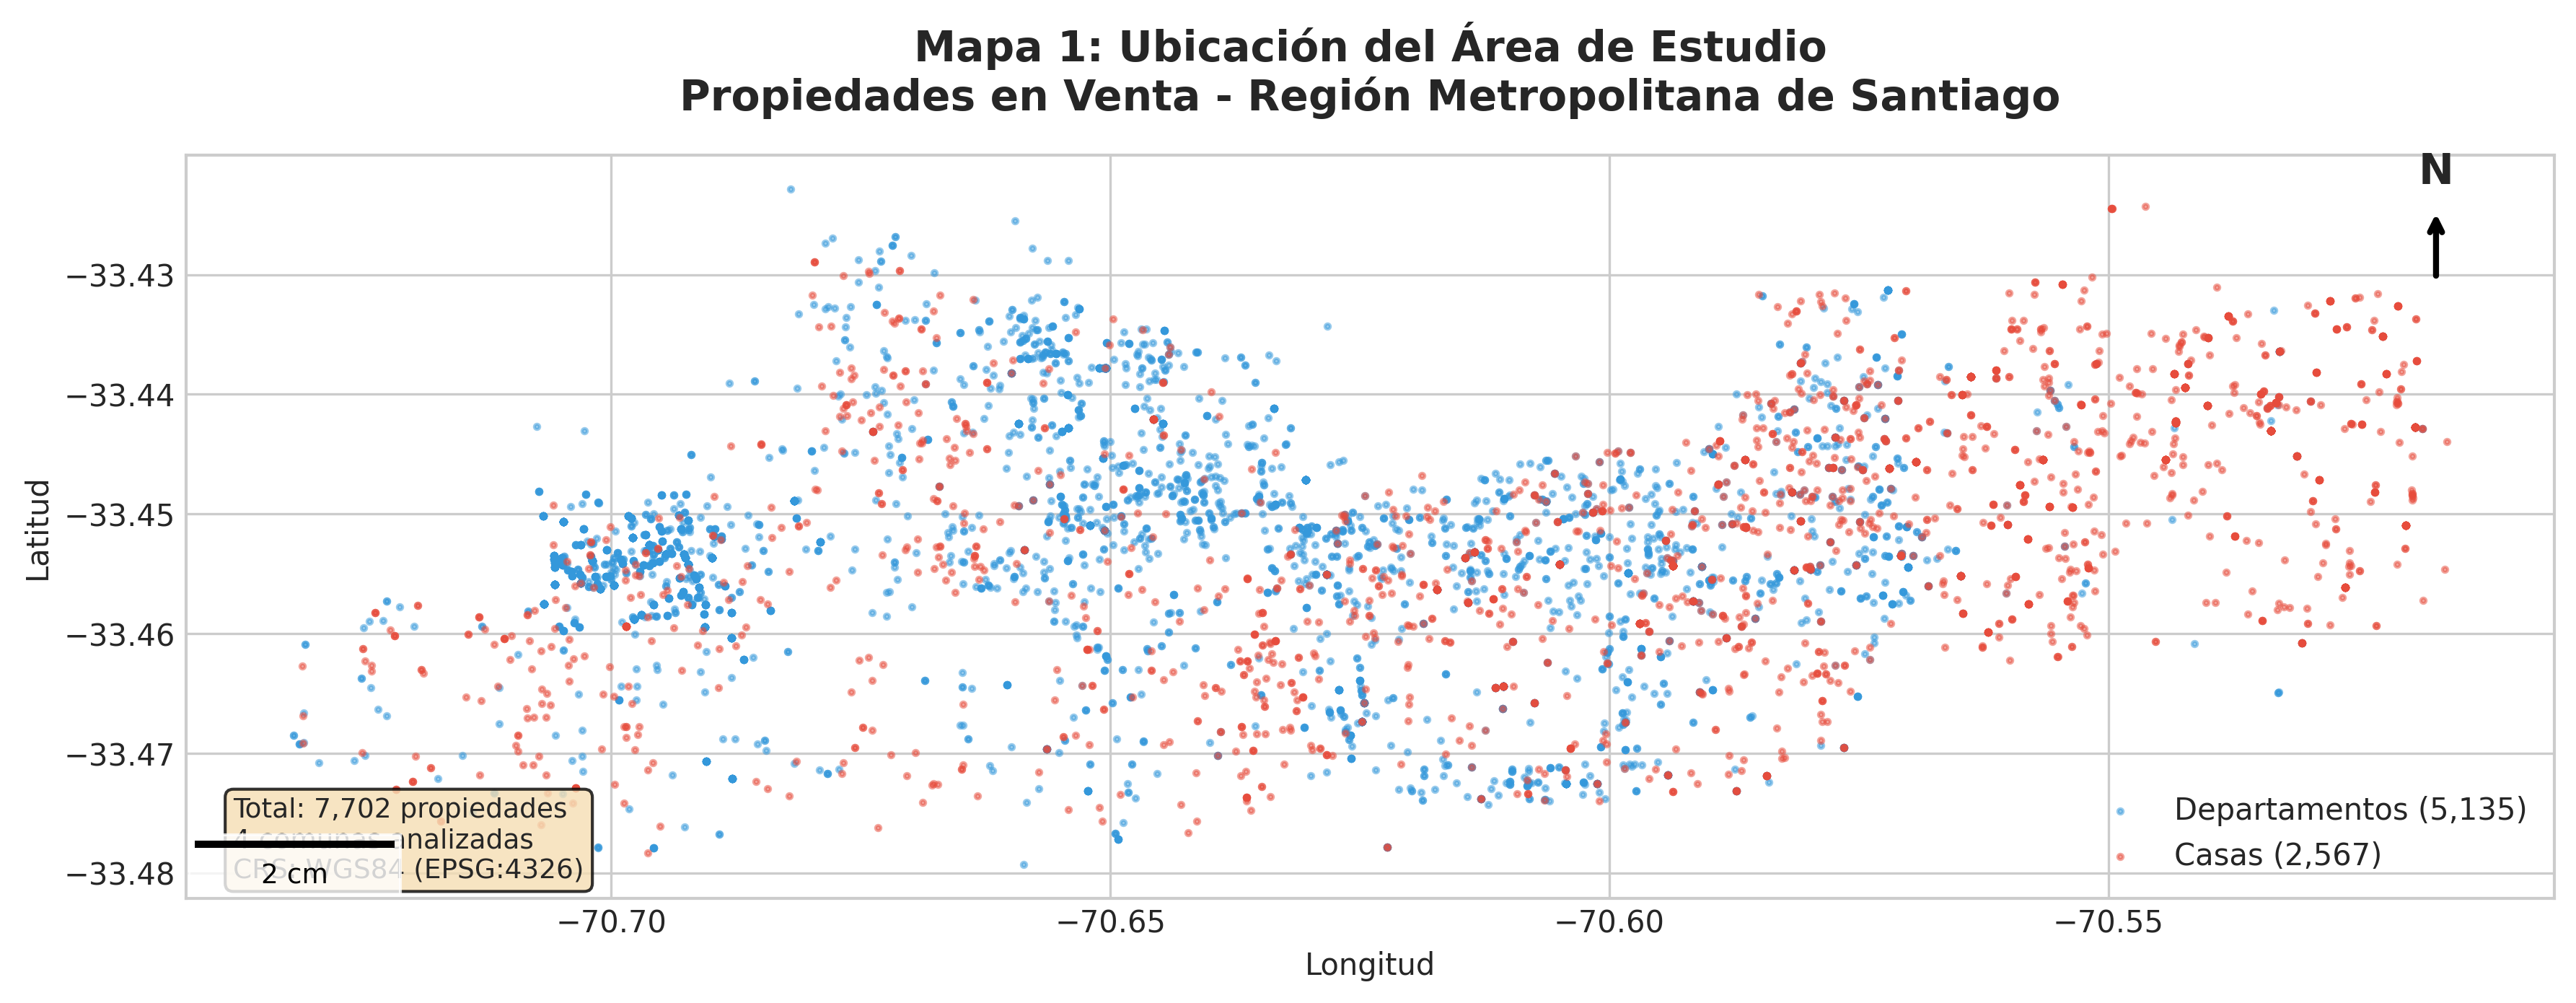
\includegraphics[width=0.8\textwidth]{figuras/mapa_01_ubicacion_area_estudio.png}
    \caption{Mapa de ubicación del área de estudio (4 comunas: Estación Central, La Reina, Ñuñoa y Santiago Centro)}
    \label{fig:ubicacion_area}
\end{figure}

\subsection{Características del Territorio}

\subsubsection{Características Físicas}

% Topografía, clima, hidrografía, etc.
\begin{itemize}
    \item \textbf{Estacion Central:}
    El territorio de Estación Central se encuentra emplazado en la unidad geomorfológica de Cuenca de Santiago y presenta un clima mediterráneo de lluvia invernal (Csb) según la clasificación de Köppen.
 La comuna pertenece a la cuenca hidrográfica del río Maipo y alberga cuerpos de agua como el Zanjón de la Aguada y el Canal Ortuzano.
 A pesar de su urbanización extensa, no existen zonas naturales sin intervención humana, y no forma parte de ningún parque natural.
 
 La comuna ha experimentado un intenso proceso de construcción en altura, especialmente desde mediados de la década de 2010, con la proliferación de megaedificios de más de 20 pisos, algunos con hasta 50 departamentos por piso, lo que ha generado críticas por condiciones de hacinamiento, colapso del sistema de alcantarillado, sombra permanente y falta de áreas verdes.
    \item \textbf{La Reina:}
    La comuna de La Reina se encuentra emplazada en las unidades geomorfológicas de Cordillera andina de retención crionival y Cuenca de Santiago. Al ubicarse a los pies de la precordillera de Los Andes o sierra de Ramón, La Reina presenta un relieve con elevadas pendientes en el oriente, producidas por la falla de Ramón, las que se moderan a medida que se avanza hacia el poniente de la comuna. Esta situación, en conjunto con el hecho de acoger diversos cursos de agua, ya sean estos canales o vertientes naturales, expone a algunos sectores de esta comuna a desbordes e incluso ocasionales aluviones, como los ocurridos en 1993 en el canal San Ramón.

La comuna presenta según la clasificación climática de Köppen clima mediterráneo de lluvia invernal (Csb), clima mediterráneo de lluvia invernal de altura (Csb (h)) y clima semiárido de lluvia invernal (BSk (s)). Esta además se halla en la cuenca hidrográfica de río Maipo. Además, la comuna posee diversos cuerpos de agua, entre los que se destacan la laguna Parque Padre Hurtado.

Áreas verdes

Vista de la parte oriental de la plaza Ossandón, en el barrio homónimo; es la principal de la comuna.
La comuna cuenta con parques y plazas, como el Parque Mahuida y el Parque Padre Hurtado, junto con el Parque Alcalde Ricardo Conteras Bueras, el Parque Quinchamalí, el Parque Andacollo, el Parque Quillagua, el Parque Tobalaba, el Parque Sánchez Fontecilla y el Parque natural Aguas de Ramón. Entre otras
    
    \item \textbf{Ñuñoa:}
    
    Clima
Según la clasificación climática de Köppen, Ñuñoa tiene un clima mediterráneo (Csb), con veranos secos y cálidos e inviernos templados con lluvias estacionales. La temperatura media anual ronda los 15/16 Celcius, y la precipitación promedio anual es de aproximadamente 340–380 mm, concentrada principalmente entre mayo y agosto.

Hidrografía y Ecosistemas
La comuna pertenece a la cuenca hidrográfica del río Maipo y posee algunos cuerpos de agua como el canal San Carlos. Históricamente, la zona albergaba ecosistemas como el bosque espinoso mediterráneo andino (con especies como Acacia caven y Baccharis paniculata), aunque actualmente no existen zonas naturales sin intervención humana debido a la total urbanización del territorio. Hasta 2022, Ñuñoa no contaba con áreas destinadas a la protección ambiental.

    \item \textbf{Santiago Centro:}
    Clima
Presenta un clima mediterráneo (Csb) según la clasificación de Köppen, con veranos secos y cálidos, e inviernos templados con precipitaciones estacionales La temperatura media anual ronda los 15 Celcius.

Hidrografía y Ecosistemas
Pertenece a la cuenca del río Maipo. Los principales cuerpos de agua son el río Mapocho y el Zanjón de la Aguada. Históricamente, albergaba ecosistemas como el bosque espinoso mediterráneo interior (Acacia caven, Prosopis chilensis), pero no existen zonas naturales sin intervención humana debido a la total urbanización. Hasta 2022, no contaba con áreas destinadas a la protección ambiental.
    
\end{itemize}
    
\subsubsection{Características Socioeconómicas}

\begin{itemize}
    \item \textbf{Estación Central:} Población aproximada de 206.792 habitantes (Censo 2017). Comuna de carácter principalmente residencial y comercial, con alta densidad poblacional debido a la proliferación de edificios en altura. Presenta estratos socioeconómicos diversos, predominando los grupos C3 y D. Es un importante nodo de transporte con el Terminal de Buses Alameda y la estación intermodal. El ingreso promedio mensual de los hogares se ubica en torno a \$650.000 CLP.
    
    \item \textbf{La Reina:} Población aproximada de 96.762 habitantes (Censo 2017). Comuna residencial de estratos medio-alto y alto (grupos ABC1 y C2), caracterizada por viviendas unifamiliares y baja densidad poblacional. Presenta altos índices de áreas verdes per cápita y calidad de vida. El ingreso promedio mensual de los hogares supera los \$2.500.000 CLP, siendo una de las comunas con mayor poder adquisitivo de la Región Metropolitana.
    
    \item \textbf{Ñuñoa:} Población aproximada de 250.192 habitantes (Censo 2017). Comuna mixta con sectores residenciales tradicionales y zonas de densificación reciente. Presenta diversidad socioeconómica con predominio de estratos medios (C2 y C3). Destaca por su oferta cultural, gastronómica y comercial. El ingreso promedio mensual de los hogares ronda los \$1.200.000 CLP. Ha experimentado un importante crecimiento inmobiliario en la última década.
    
    \item \textbf{Santiago Centro:} Población aproximada de 503.147 habitantes (Censo 2017). Centro histórico, financiero y comercial de la ciudad. Alta densidad poblacional con predominio de departamentos. Presenta gran diversidad socioeconómica, desde sectores populares hasta zonas renovadas de estratos medios. Concentra servicios gubernamentales, comercio, universidades y actividad económica terciaria. El ingreso promedio mensual de los hogares es de aproximadamente \$800.000 CLP.
\end{itemize}

\subsection{Justificación de la Selección}

La selección de estas cuatro comunas responde a criterios metodológicos y prácticos que permiten un análisis representativo del mercado inmobiliario de Santiago:

\begin{enumerate}
    \item \textbf{Diversidad socioeconómica:} Las comunas seleccionadas representan un espectro amplio de niveles socioeconómicos, desde La Reina (estrato alto) hasta Estación Central (estratos medio-bajo), pasando por Ñuñoa y Santiago Centro (estratos medios). Esta diversidad permite evaluar cómo varían los factores de satisfacción residencial según el contexto socioeconómico.
    
    \item \textbf{Heterogeneidad urbana:} El área de estudio incluye zonas de alta densificación vertical (Estación Central, Santiago Centro), sectores residenciales tradicionales (La Reina), y comunas en transición con mezcla de tipologías (Ñuñoa). Esto permite analizar el impacto de diferentes morfologías urbanas en la satisfacción residencial.
    
    \item \textbf{Disponibilidad de datos:} Estas comunas presentan un volumen significativo de propiedades en venta (7.702 propiedades), lo que garantiza una muestra estadísticamente robusta para el entrenamiento y validación de los modelos predictivos.
    
    \item \textbf{Conectividad y servicios:} Las cuatro comunas cuentan con cobertura de la red de Metro de Santiago y acceso a diversos servicios urbanos, permitiendo evaluar el impacto de la accesibilidad en la satisfacción residencial.
    
    \item \textbf{Contigüidad geográfica:} La cercanía espacial de las comunas facilita el análisis de efectos de borde y la comparación de condiciones similares de entorno metropolitano, minimizando sesgos por diferencias macro-regionales.
\end{enumerate} 

% ====================================================================
% 4. DATOS Y METODOLOGÍA
% ====================================================================

